% !TeX program = xelatex
% !TeX encoding = UTF-8
% Spedizione P10 · Un’analisi ricostruibile e verificabile
% Presentazione della spedizione P10 nella serie planetaria di GeoStat Lab.
% Compilazione: xelatex -interaction=nonstopmode P10_Ricostruibile.tex (due passaggi)
% 26 slide. Diagrammi TikZ, figure vettoriali da R/P10_figure.R, codice R, dati ed esperimenti inclusi.
\RequirePackage{fix-cm}
\documentclass[12pt,aspectratio=1610]{beamer}
\geometry{paperwidth=20cm,paperheight=12.5cm}
\usepackage[italian,provide=*]{babel}
\usepackage{fontspec,adjustbox,tabularx}
\IfFontExistsTF{NimbusSans-Regular.otf}{
\setsansfont{NimbusSans-Regular.otf}[BoldFont=NimbusSans-Bold.otf,ItalicFont=NimbusSans-Italic.otf,BoldItalicFont=NimbusSans-BoldItalic.otf]
\setmainfont{NimbusSans-Regular.otf}[BoldFont=NimbusSans-Bold.otf,ItalicFont=NimbusSans-Italic.otf,BoldItalicFont=NimbusSans-BoldItalic.otf]
}{
\setsansfont{TeX Gyre Heros}
\setmainfont{TeX Gyre Heros}
}
\IfFontExistsTF{DejaVu Sans Mono}{
\setmonofont{DejaVu Sans Mono}[Scale=.88]
}{\setmonofont{Latin Modern Mono}[Scale=.88]}
\usefonttheme{professionalfonts}
\usepackage{amsmath,amssymb,booktabs,array,graphicx,tikz,bookmark}
\usetikzlibrary{calc,positioning,arrows.meta}
\graphicspath{{Figure/}}
\definecolor{Paper}{HTML}{F8F6F1}
\definecolor{Ink}{HTML}{253344}
\definecolor{Navy}{HTML}{15283E}
\definecolor{Quantum}{HTML}{5146A5}
\definecolor{Classical}{HTML}{087C74}
\definecolor{Muted}{HTML}{657180}
\definecolor{Rule}{HTML}{D6DAD9}
\definecolor{Night}{HTML}{112236}
\definecolor{Lilac}{HTML}{ABB5FF}
\definecolor{Mint}{HTML}{72D8C8}
\setbeamercolor{background canvas}{bg=Paper}
\setbeamercolor{normal text}{fg=Ink}
\setbeamertemplate{navigation symbols}{}
\setbeamertemplate{headline}{}
\setbeamertemplate{footline}{}
\setbeamersize{text margin left=0pt,text margin right=0pt}
\hypersetup{colorlinks=true,linkcolor=Classical,urlcolor=Classical,pdfpagemode=UseOutlines,pdfstartview=Fit,
 pdftitle={Spedizione P10 · Un’analisi ricostruibile e verificabile},pdfauthor={GeoStat Lab · materiali di Marzio De Corato},
 pdfsubject={GeoStat Lab · P10}}
\bookmarksetup{open,openlevel=0,depth=2}
\newsavebox{\BodyBox}
\newsavebox{\SideBox}
\newsavebox{\RecallBox}
\newsavebox{\TitleBox}
\newcommand{\MeasureBox}[2]{\typeout{REVIEWBOX:#1:\the\wd#2:\the\ht#2:\the\dp#2}}

% Revisione completa: diagrammi TikZ, formalismo e box R.
\usepackage[most]{tcolorbox}
\usepackage{listings}
\usetikzlibrary{fit,backgrounds,matrix,decorations.pathreplacing}
\definecolor{GeoA}{HTML}{1D7890}
\definecolor{GeoB}{HTML}{C57E42}
\definecolor{GeoC}{HTML}{7363AA}
\definecolor{GeoTint}{HTML}{F0F4F3}
\lstdefinestyle{GeoR}{language=R,basicstyle=\ttfamily\fontsize{9.2}{12.2}\selectfont,
 keywordstyle=\color{Quantum}\bfseries,commentstyle=\color{Classical},stringstyle=\color{GeoB},
 numbers=left,numberstyle=\tiny\color{Muted},numbersep=4pt,showstringspaces=false,
 columns=fullflexible,keepspaces=true,breaklines=true,xleftmargin=1.15em,
 frame=none,aboveskip=0pt,belowskip=0pt,tabsize=2}
\newsavebox{\PilotLeftBox}
\newsavebox{\PilotRightBox}
\newcommand{\PLabel}[1]{\par{\color{Classical}\bfseries\fontsize{9}{11}\selectfont\MakeUppercase{#1}}\par\vspace{1.8mm}}
\newcommand{\PBody}[1]{\par{\fontsize{11.3}{14.8}\selectfont #1\par}}
\newcommand{\PSmall}[1]{\par{\fontsize{9.8}{13.1}\selectfont #1\par}}
\newcommand{\PCode}[2]{%
\begin{tcolorbox}[enhanced,arc=1.8mm,boxrule=.65pt,
  colback=white,colframe=Classical!75!Navy,colbacktitle=Navy,
  coltitle=white,fonttitle=\bfseries\fontsize{9.6}{12}\selectfont,
  title={#1},left=1.7mm,right=1.3mm,top=1.5mm,bottom=1.3mm,
  before skip=1mm,after skip=1mm]
\lstinputlisting[style=GeoR]{Codice/#2}
\end{tcolorbox}}
\newcommand{\PInfo}[1]{%
\begin{tcolorbox}[enhanced,arc=1.6mm,boxrule=.55pt,colback=GeoTint,
 colframe=Rule!80!Classical,left=2.3mm,right=2.3mm,top=2mm,bottom=2mm,
 before skip=1mm,after skip=1mm]
\PSmall{#1}\end{tcolorbox}}
\tikzset{
 pFlow/.style={draw=Classical!45,fill=white,rounded corners=2mm,
  line width=.7pt,align=center,minimum height=1.1cm,font=\sffamily\fontsize{10}{12}\selectfont},
 pEdge/.style={-{Latex[length=2.3mm]},draw=Classical,line width=.95pt},
 pGroup/.style={draw=Rule,fill=white,rounded corners=2mm,line width=.65pt},
 pDotA/.style={circle,fill=GeoA,inner sep=1.25pt},
 pDotB/.style={circle,fill=GeoB,inner sep=1.25pt},
 pDotC/.style={circle,fill=GeoC,inner sep=1.25pt}
}
\newcommand{\PilotChrome}[4]{%
  \node[anchor=north west,inner sep=0,text width=17.7cm] at ([xshift=.95cm,yshift=-.55cm]current page.north west) {\color{Navy}\bfseries\fontsize{20.6}{24.5}\selectfont #1};
  \node[anchor=north east,inner sep=0] at ([xshift=19.05cm,yshift=-.14cm]current page.north west) {\color{Classical}\fontsize{8}{10}\selectfont\hyperlink{slide2}{#2}};
  \draw[Classical,line width=1.2pt] ([xshift=.95cm,yshift=-1.7cm]current page.north west)--([xshift=2.35cm,yshift=-1.7cm]current page.north west);
  \draw[Rule,line width=.65pt] ([xshift=.95cm,yshift=-10.36cm]current page.north west)--([xshift=19.05cm,yshift=-10.36cm]current page.north west);
  \node[anchor=north west,inner sep=0] at ([xshift=.96cm,yshift=-10.55cm]current page.north west) {\color{Classical}\bfseries\fontsize{9.1}{12}\selectfont DA RICORDARE};
  \node[anchor=north west,inner sep=0,text width=14.3cm] at ([xshift=4.2cm,yshift=-10.53cm]current page.north west) {\color{Ink}\fontsize{10.3}{13.8}\selectfont #4};
  \draw[Rule,line width=.35pt] ([xshift=.95cm,yshift=-11.92cm]current page.north west)--([xshift=19.05cm,yshift=-11.92cm]current page.north west);
  \node[anchor=north west,inner sep=0] at ([xshift=.95cm,yshift=-12.06cm]current page.north west) {\color{Muted}\fontsize{7.7}{9.2}\selectfont Spedizione P10 · Un’analisi ricostruibile e verificabile};
  \node[anchor=north east,inner sep=0] at ([xshift=19.05cm,yshift=-12.06cm]current page.north west) {\color{Muted}\fontsize{7.7}{9.2}\selectfont #3/26};
}


% Stili comuni per i diagrammi scientifici della revisione completa.
\tikzset{
 pAxis/.style={-{Latex[length=2mm]},draw=Muted,line width=.65pt},
 pNote/.style={font=\sffamily\fontsize{9}{11.5}\selectfont,text=Muted,align=center},
 pLabel/.style={font=\sffamily\fontsize{10}{12.5}\selectfont,text=Ink,align=center}
}
\newsavebox{\FullWideBox}
\setlength{\emergencystretch}{1em}




\newcommand{\PLab}[2]{\par{\color{Classical}\bfseries\fontsize{9}{11}\selectfont
\href{#1}{\MakeUppercase{#2}}}\par\vspace{1.8mm}}

\definecolor{Measure}{HTML}{A05B10}\definecolor{Rose}{HTML}{9B4564}\definecolor{Wash}{HTML}{EAE7F6}\definecolor{Gold}{HTML}{EEC184}
\tikzset{arr/.style={-{Stealth[length=2mm]},line width=.8pt,draw=Classical}}
\newcommand{\Colonna}[2]{\begin{adjustbox}{max totalsize={#1}{7.95cm},valign=t}\begin{minipage}[t]{#1}\raggedright\fontsize{11.3}{14.8}\selectfont #2\end{minipage}\end{adjustbox}}
\begin{document}

\begin{frame}[plain]\hypertarget{slide1}{}\bookmark[level=0,page=1]{Spedizione P10}
\begin{tikzpicture}[remember picture,overlay]
\fill[Night](current page.south west) rectangle(current page.north east);
\IfFileExists{Scena/copertina.jpg}{\node[inner sep=0] at(current page.center){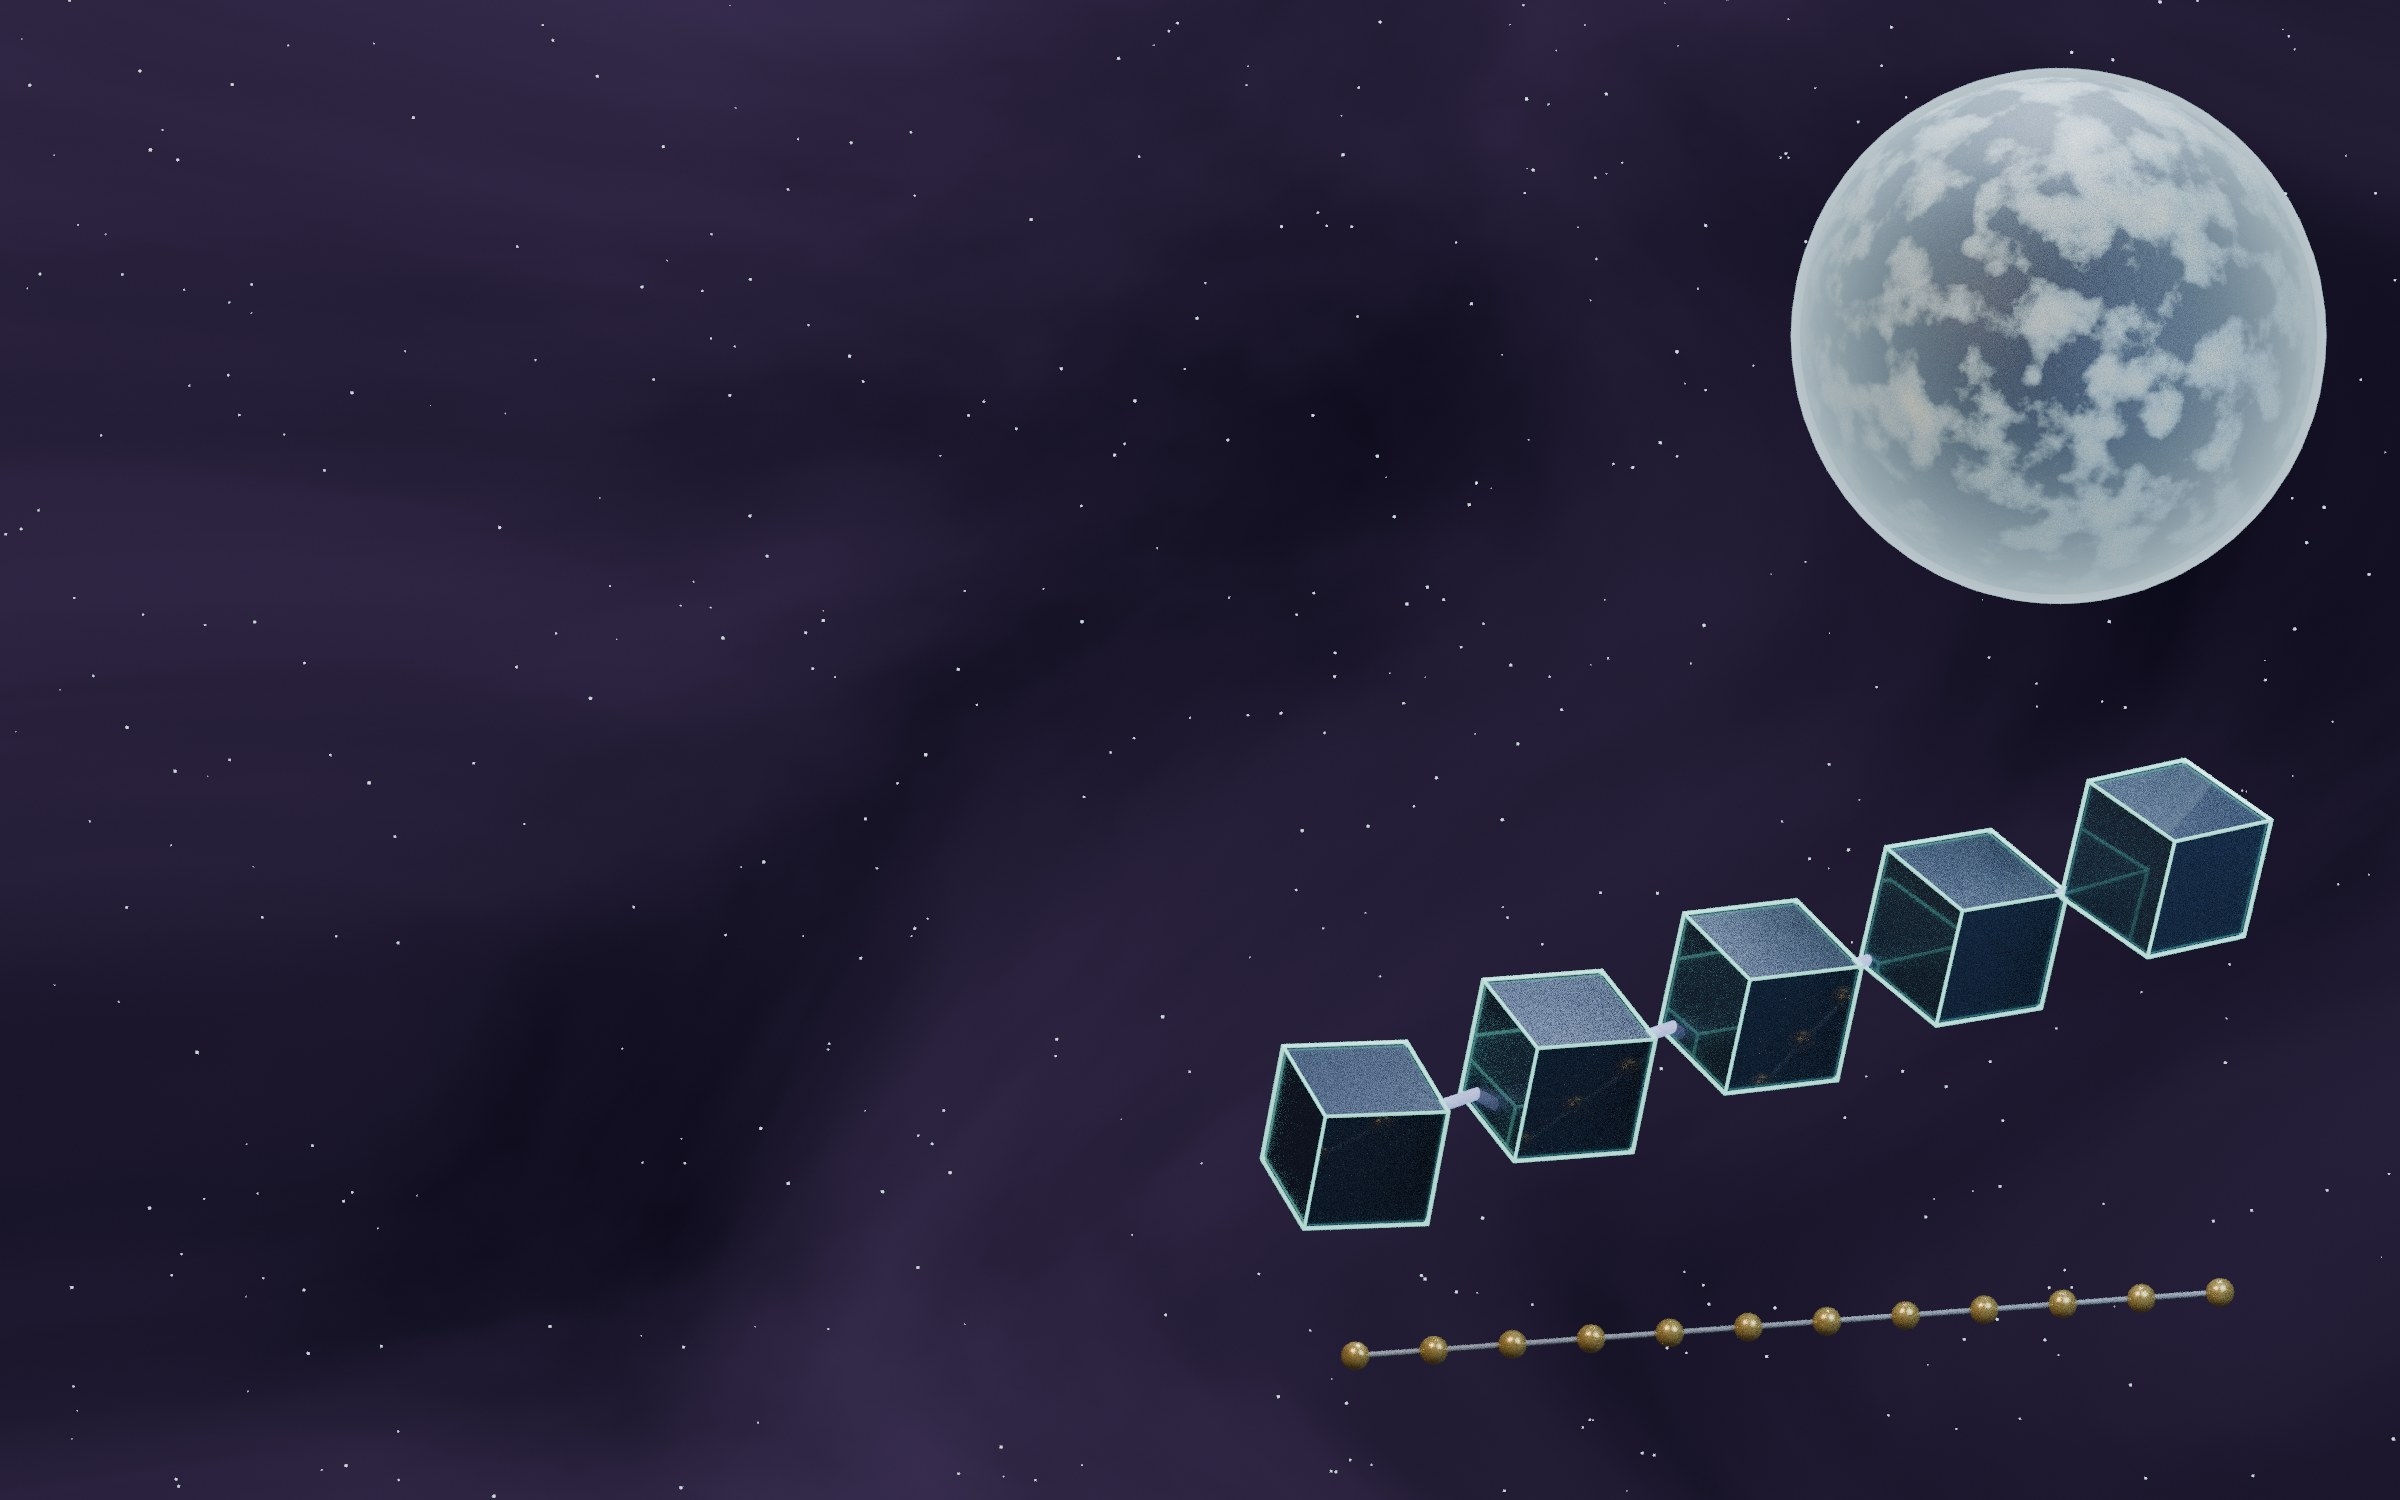
\includegraphics[width=20cm,height=12.5cm]{Scena/copertina.jpg}};}{}
\node[anchor=north west,inner sep=0] at([xshift=1.05cm,yshift=-1.10cm]current page.north west){\color{Mint}\bfseries\fontsize{23}{28}\selectfont SPEDIZIONE P10};
\node[anchor=north west,inner sep=0] at([xshift=1.07cm,yshift=-2.16cm]current page.north west){\color{white}\fontsize{9}{12}\selectfont MACROPROGETTO P10 · SCIENZE DELLA TERRA};
\draw[Mint,line width=1.5pt]([xshift=1.07cm,yshift=-2.78cm]current page.north west)--([xshift=2.6cm,yshift=-2.78cm]current page.north west);
\node[anchor=north west,inner sep=0] at([xshift=1.05cm,yshift=-3.35cm]current page.north west){\begin{minipage}{9.2cm}\raggedright\color{white}\bfseries\fontsize{28.5}{34.5}\selectfont Un’analisi\\ricostruibile\\e verificabile\end{minipage}};
\node[anchor=north west,inner sep=0] at([xshift=1.07cm,yshift=-7.88cm]current page.north west){\begin{minipage}{8.9cm}\raggedright\color{Lilac}\fontsize{12.2}{17}\selectfont Ventiquattro provini, sei stazioni\end{minipage}};
\node[anchor=north west,inner sep=0] at([xshift=1.07cm,yshift=-8.70cm]current page.north west){\begin{minipage}{8.9cm}\raggedright\color{white!75}\fontsize{10.3}{14.5}\selectfont Dati immutati, funzioni, controlli numerici e storia delle modifiche\end{minipage}};
\node[anchor=north west,inner sep=0] at([xshift=1.07cm,yshift=-10.52cm]current page.north west){\color{white}\fontsize{10.5}{14}\selectfont GeoStat Lab · corso di Marzio De Corato};
\node[anchor=north west,inner sep=0] at([xshift=1.07cm,yshift=-11.17cm]current page.north west){\color{Mint}\fontsize{8.8}{11}\selectfont\href{https://creativecommons.org/licenses/by-nc-sa/4.0/}{Impaginazione da Tessera · CC BY-NC-SA 4.0}};
\end{tikzpicture}\end{frame}

\begin{frame}[plain]\hypertarget{slide2}{}
\bookmark[level=1,page=2]{Indice della presentazione}
\begin{tikzpicture}[remember picture,overlay]
\PilotChrome{Indice della presentazione}{PERCORSO}{2}{I titoli dell’indice aprono i capitoli. Il nome del capitolo in alto riporta a questa pagina.}
\node[anchor=north west,inner sep=0] at([xshift=.96cm,yshift=-2.12cm]current page.north west){\Colonna{9.40cm}{\PLabel{Capitoli}
{\fontsize{10.7}{13.5}\selectfont\hyperlink{slide4}{Dati e trasformazioni dichiarate\hfill 4}\par}\vspace{.16cm}
{\fontsize{10.7}{13.5}\selectfont\hyperlink{slide9}{Prove del codice e integrità dei file\hfill 9}\par}\vspace{.16cm}
{\fontsize{10.7}{13.5}\selectfont\hyperlink{slide14}{Piani casuali, versioni e consegna\hfill 14}\par}\vspace{.16cm}
{\fontsize{10.7}{13.5}\selectfont\hyperlink{slide18}{Laboratori della spedizione\hfill 18}\par}\vspace{.16cm}

}};
\node[anchor=north west,inner sep=0] at([xshift=10.85cm,yshift=-2.12cm]current page.north west){\Colonna{8.16cm}{\PLabel{Percorso di lettura}
\PBody{Il percorso dichiara dati e trasformazioni, mette alla prova funzioni e file con controlli numerici e impronte, conserva piani casuali e storia delle versioni. I laboratori finali riprendono le tre fasi della spedizione.}
\PInfo{Le pagine Scenario A e Confronto riprendono gli esperimenti nel browser con dati sintetici. I valori di partenza del simulatore differiscono da quelli del caso.}
\href{https://marzione00.github.io/Lab_Geo/\#modulo-P10}{\color{Classical}\bfseries Apri la spedizione P10 su GeoStat Lab}
}};
\end{tikzpicture}\end{frame}

\begin{frame}[plain]\hypertarget{slide3}{}
\bookmark[level=1,page=3]{Che cosa serve perché un’analisi semplice possa essere rieseguita e verificata da altri?}
\begin{tikzpicture}[remember picture,overlay]
\PilotChrome{{\fontsize{15.3}{19}\selectfont Che cosa serve perché un’analisi semplice possa essere rieseguita e verificata da altri?}}{IL CASO GUIDA}{3}{La copertina è una scena illustrativa: i blocchi rappresentano i passaggi dell’analisi, i punti dorati le versioni.}
\node[anchor=north west,inner sep=0] at([xshift=.96cm,yshift=-2.12cm]current page.north west){\Colonna{9.40cm}{{\centering\resizebox{0.97\linewidth}{!}{\begin{tikzpicture}[x=1cm,y=1cm,every node/.style={font=\sffamily\fontsize{10}{12}\selectfont,text=Ink}]
\draw[draw=Classical,fill=Classical!8,rounded corners=2mm,line width=.7pt] (0,0.00) rectangle (8.6,-0.78);
\node[circle,anchor=center,fill=Classical,inner sep=0,minimum size=.5cm,text=white,font=\sffamily\bfseries\fontsize{9}{10}\selectfont] at (.48,-0.39) {1};
\node[anchor=west,text width=7.4cm,align=left] at (.95,-0.39) {Dati e trasformazioni dichiarate};
\draw[pEdge] (.48,-0.80)--(.48,-1.02);
\draw[draw=Classical,fill=Classical!8,rounded corners=2mm,line width=.7pt] (0,-1.04) rectangle (8.6,-1.82);
\node[circle,anchor=center,fill=Classical,inner sep=0,minimum size=.5cm,text=white,font=\sffamily\bfseries\fontsize{9}{10}\selectfont] at (.48,-1.43) {2};
\node[anchor=west,text width=7.4cm,align=left] at (.95,-1.43) {Prove del codice e integrità dei file};
\draw[pEdge] (.48,-1.84)--(.48,-2.06);
\draw[draw=Classical,fill=Classical!8,rounded corners=2mm,line width=.7pt] (0,-2.08) rectangle (8.6,-2.86);
\node[circle,anchor=center,fill=Classical,inner sep=0,minimum size=.5cm,text=white,font=\sffamily\bfseries\fontsize{9}{10}\selectfont] at (.48,-2.47) {3};
\node[anchor=west,text width=7.4cm,align=left] at (.95,-2.47) {Piani casuali, versioni e consegna};
\draw[pEdge] (.48,-2.88)--(.48,-3.10);
\draw[draw=GeoB,fill=GeoB!8,rounded corners=2mm,line width=.7pt] (0,-3.12) rectangle (8.6,-3.90);
\node[circle,anchor=center,fill=GeoB,inner sep=0,minimum size=.5cm,text=white,font=\sffamily\bfseries\fontsize{9}{10}\selectfont] at (.48,-3.51) {L};
\node[anchor=west,text width=7.4cm,align=left] at (.95,-3.51) {Laboratori della spedizione};
\end{tikzpicture}
}\par}
\PSmall{Capitoli della spedizione; L indica i laboratori conclusivi.}
}};
\node[anchor=north west,inner sep=0] at([xshift=10.85cm,yshift=-2.12cm]current page.north west){\Colonna{8.16cm}{\PLabel{Il caso}
\PBody{Ventiquattro provini di sei stazioni forniscono massa e volume, da cui si ricava la densità. La quantità fisica è semplice, così che l’attenzione cada su dati, funzioni, controlli, impronte dei file e storia delle modifiche.}
\PInfo{Seguiremo la densità dalla tabella immutata alla funzione con il suo contratto, ai test con errori deliberati, fino alla consegna con versioni e dipendenze.}
}};
\end{tikzpicture}\end{frame}

\begin{frame}[plain]\hypertarget{slide4}{}
\bookmark[level=0,page=4]{Dati e trasformazioni dichiarate}
\bookmark[level=1,page=4]{La riproducibilità riguarda l’intero procedimento}
\begin{tikzpicture}[remember picture,overlay]
\PilotChrome{La riproducibilità riguarda l’intero procedimento}{DATI E TRASFORMAZIONI DICHIARATE}{4}{La ricostruzione del calcolo deve conservare dati, trasformazioni, ambiente e significato della quantità stimata.}
\node[anchor=north west,inner sep=0] at([xshift=.96cm,yshift=-2.12cm]current page.north west){\Colonna{9.40cm}{{\centering\resizebox{0.90\linewidth}{!}{\begin{tikzpicture}[x=1cm,y=-.87cm,every node/.style={font=\fontsize{12.2}{15}\selectfont,text=Ink},arr/.style={-{Stealth[length=2mm]},line width=.8pt,draw=Classical}]\path[use as bounding box] (0,0) rectangle (7.45,6.2);
\draw[draw=Classical,fill=Classical!8,rounded corners=2pt,line width=.7pt] (0.7,0.7) rectangle (3.2,2.1);
\node[anchor=center,text=Ink,font=\fontsize{13}{15}\selectfont,text width=2.2cm,align=center] at (1.95,1.4) {Dati e unità};
\draw[draw=Quantum,fill=Quantum!8,rounded corners=2pt,line width=.7pt] (4.1,0.7) rectangle (6.6,2.1);
\node[anchor=center,text=Ink,font=\fontsize{12}{15}\selectfont,text width=2.2cm,align=center] at (5.35,1.4) {Codice e ambiente};
\draw[arr,draw=Classical] (2,2.4)--(3.2,3.3);
\draw[arr,draw=Quantum] (5.3,2.4)--(4.2,3.3);
\draw[draw=Classical,fill=Classical!8,rounded corners=2pt,line width=.7pt] (1.2,3.6) rectangle (6.2,5);
\node[anchor=center,text=Ink,font=\fontsize{13}{15}\selectfont,text width=4.7cm,align=center] at (3.7,4.3) {Risultato verificabile};
\node[anchor=center,text=Ink,font=\fontsize{11}{15}\selectfont,text width=6.8cm,align=center] at (3.7,6) {La conclusione conserva anche le ipotesi scientifiche.};

\end{tikzpicture}}\par}
}};
\node[anchor=north west,inner sep=0] at([xshift=10.85cm,yshift=-2.12cm]current page.north west){\Colonna{8.16cm}{\PBody{Il progetto ricostruisce la densità di ventiquattro provini e ne calcola la media nelle sei stazioni di provenienza. La quantità fisica è semplice, così che l’attenzione possa concentrarsi su provenienza dei dati, funzioni, verifiche ed esportazione dei risultati. Ogni passaggio viene conservato in forma eseguibile e accompagnato dalle condizioni che ne determinano il significato. Ottenere nuovamente lo stesso numero dimostra la stabilità del procedimento dichiarato, mentre la validità della misura e della conclusione geologica richiede anche un’adeguata definizione del problema.}
}};
\end{tikzpicture}\end{frame}

\begin{frame}[plain]\hypertarget{slide5}{}
\bookmark[level=1,page=5]{Il contratto dei dati precede il calcolo}
\begin{tikzpicture}[remember picture,overlay]
\PilotChrome{Il contratto dei dati precede il calcolo}{DATI E TRASFORMAZIONI DICHIARATE}{5}{Un contratto esplicito permette di distinguere un input inammissibile da un risultato inatteso ma valido.}
\node[anchor=north west,inner sep=0] at([xshift=.96cm,yshift=-2.12cm]current page.north west){\Colonna{9.40cm}{\PBody{La funzione di validazione richiede identificativi unici, stazioni presenti, masse e volumi numerici, finiti e strettamente positivi. Tali condizioni definiscono il dominio ammissibile dell’operazione, poiché una divisione formalmente eseguibile potrebbe altrimenti produrre risultati fisicamente incoerenti. La validazione restituisce la tabella controllata, che passa alla trasformazione successiva. Il dato originario rimane conservato e ogni correzione sostanziale dovrebbe essere documentata nella fonte, evitando sostituzioni implicite durante il calcolo.}
\par\smallskip{\centering\adjustbox{max width=.98\linewidth}{$\displaystyle m_i,V_i\in\mathbb R_{>0}\quad\forall i,\qquad id_i\ne id_j\quad(i\ne j)$}\par\smallskip}
}};
\node[anchor=north west,inner sep=0] at([xshift=10.85cm,yshift=-2.12cm]current page.north west){\Colonna{8.16cm}{\PInfo{$m_i$: massa in g; $V_i$: volume in cm³; $id_i$: identificativo del provino. Si richiedono anche schema valido e stazione presente. Finitezza e positività escludono NA, NaN e infiniti. Gli identificativi sono unici; la stazione si ripete perché raggruppa provini distinti.}
}};
\end{tikzpicture}\end{frame}

\begin{frame}[plain]\hypertarget{slide6}{}
\bookmark[level=1,page=6]{La funzione compone operazioni con un significato}
\begin{tikzpicture}[remember picture,overlay]
\PilotChrome{La funzione compone operazioni con un significato}{DATI E TRASFORMAZIONI DICHIARATE}{6}{La composizione è definita anche dai tipi di oggetto restituiti e dall’unità rappresentata in ogni passaggio.}
\node[anchor=north west,inner sep=0] at([xshift=.96cm,yshift=-2.12cm]current page.north west){\Colonna{9.40cm}{{\centering\resizebox{0.90\linewidth}{!}{\begin{tikzpicture}[x=1cm,y=-.87cm,every node/.style={font=\fontsize{12.2}{15}\selectfont,text=Ink},arr/.style={-{Stealth[length=2mm]},line width=.8pt,draw=Classical}]\path[use as bounding box] (0,0) rectangle (7.45,6.2);
\draw[draw=Classical,fill=Classical!8,rounded corners=2pt,line width=.7pt] (0.6,0.6) rectangle (6.8,1.8);
\node[anchor=center,text=Ink,font=\fontsize{13}{15}\selectfont,text width=5.8cm,align=center] at (3.7,1.2) {V: tabella validata};
\draw[arr,draw=Classical] (3.7,2)--(3.7,2.5);
\draw[draw=Quantum,fill=Quantum!8,rounded corners=2pt,line width=.7pt] (0.6,2.7) rectangle (6.8,3.9);
\node[anchor=center,text=Ink,font=\fontsize{13}{15}\selectfont,text width=5.8cm,align=center] at (3.7,3.3) {T: densità dei provini};
\draw[arr,draw=Classical] (3.7,4.1)--(3.7,4.6);
\draw[draw=Classical,fill=Classical!8,rounded corners=2pt,line width=.7pt] (0.6,4.8) rectangle (6.8,6);
\node[anchor=center,text=Ink,font=\fontsize{13}{15}\selectfont,text width=5.8cm,align=center] at (3.7,5.4) {A: media per stazione};

\end{tikzpicture}}\par}
\PSmall{V: validazione; T: trasformazione; A: aggregazione. Si applica prima V. $m_i$: massa in g; $V_i$: volume in cm³; $\rho_i$: densità.}
}};
\node[anchor=north west,inner sep=0] at([xshift=10.85cm,yshift=-2.12cm]current page.north west){\Colonna{8.16cm}{\PBody{Il procedimento applica dapprima la validazione, quindi aggiunge la densità come rapporto fra massa e volume e infine aggrega per stazione. La composizione conserva la relazione fra unità fisica e unità della tabella: il rapporto è espresso in grammi per centimetro cubo, mentre la sintesi restituisce una riga per stazione. La funzione restituisce sempre un risultato ordinato per identificativo della stazione, rendendo confrontabili esecuzioni che ricevono le stesse righe in un ordine differente.}
\par\smallskip{\centering\adjustbox{max width=.98\linewidth}{$\displaystyle F=A\circ T\circ V,\qquad\rho_i=\frac{m_i}{V_i}$}\par\smallskip}
}};
\end{tikzpicture}\end{frame}

\begin{frame}[plain]\hypertarget{slide7}{}
\bookmark[level=1,page=7]{Un valore manuale controlla il risultato}
\begin{tikzpicture}[remember picture,overlay]
\PilotChrome{Un valore manuale controlla il risultato}{DATI E TRASFORMAZIONI DICHIARATE}{7}{Un controllo numerico è più informativo quando il valore atteso deriva da un ragionamento indipendente.}
\node[anchor=north west,inner sep=0] at([xshift=.96cm,yshift=-2.12cm]current page.north west){\Colonna{9.40cm}{\PBody{Il primo provino ha massa 107,2 grammi e volume quaranta centimetri cubi, da cui deriva una densità di 2,68. Per la stazione A1 la media delle quattro densità è 2,685. Questi valori vengono calcolati indipendentemente dalla funzione generale e inseriti nei controlli. Il confronto verifica così un risultato fisico elementare con un calcolo indipendente dall’istruzione del programma. La tabella originale viene controllata anche per accertare che l’aggiunta della densità riguardi soltanto l’oggetto restituito.}
}};
\node[anchor=north west,inner sep=0] at([xshift=10.85cm,yshift=-2.12cm]current page.north west){\Colonna{8.16cm}{\begin{tcolorbox}[enhanced,arc=1.7mm,boxrule=.6pt,colback=white,colframe=Classical!60!Navy,colbacktitle=Navy,coltitle=white,fonttitle=\bfseries\small,title={R · calcolo riproducibile},left=1.7mm,right=1.3mm,top=1.1mm,bottom=1.1mm,before skip=1mm,after skip=1.0mm]\lstinputlisting[style=GeoR,language=R,basicstyle=\ttfamily\fontsize{8.6}{11.4}\selectfont]{Codice/pipeline.R}\end{tcolorbox}
\PLabel{Risultato in R}
\begin{tcolorbox}[colback=GeoTint,colframe=Rule,boxrule=.5pt,arc=1.4mm,left=2mm,right=1mm,top=1mm,bottom=1mm]{\fontsize{8.4}{10.9}\selectfont\ttfamily \mbox{\ \ stazione\ densita}\\\mbox{1\ \ \ \ \ \ \ A1\ \ 2.6850}\\\mbox{6\ \ \ \ \ \ \ B3\ \ 2.5125}}\end{tcolorbox}
}};
\end{tikzpicture}\end{frame}

\begin{frame}[plain]\hypertarget{slide8}{}
\bookmark[level=1,page=8]{La sintesi conserva la variabilità entro stazione}
\begin{tikzpicture}[remember picture,overlay]
\PilotChrome{La sintesi conserva la variabilità entro stazione}{DATI E TRASFORMAZIONI DICHIARATE}{8}{La ricostruibilità della sintesi non sostituisce la giustificazione inferenziale di un confronto territoriale.}
\node[anchor=north west,inner sep=0] at([xshift=.96cm,yshift=-2.12cm]current page.north west){\Colonna{9.40cm}{{\centering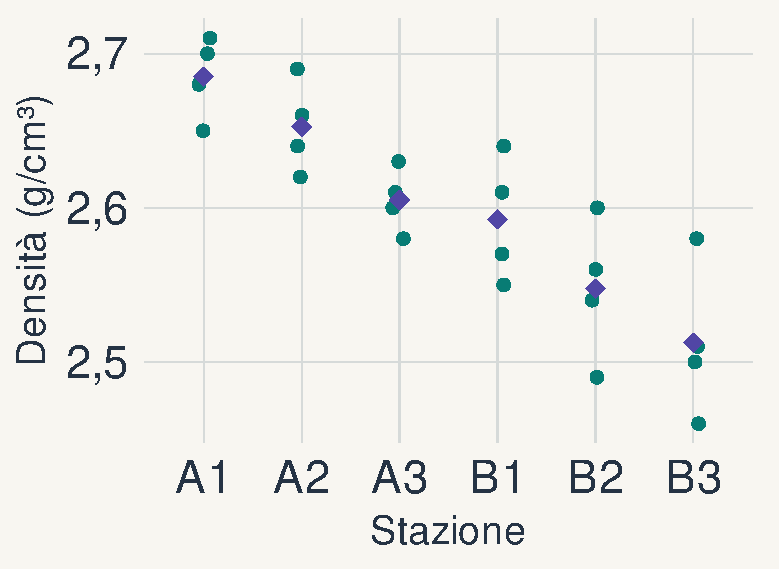
\includegraphics[width=\linewidth,height=6.15cm,keepaspectratio]{Figure/F01.pdf}\par}
\PSmall{Provini in verde e medie delle stazioni in viola.}
}};
\node[anchor=north west,inner sep=0] at([xshift=10.85cm,yshift=-2.12cm]current page.north west){\Colonna{8.16cm}{\PBody{La figura affianca le densità dei singoli provini alle medie delle sei stazioni, così che il risultato aggregato rimanga leggibile rispetto ai dati che lo determinano. Le medie vanno da 2,5125 a 2,685 grammi per centimetro cubo, mentre la media dei ventiquattro provini è circa 2,59917. I rombi indicano valori descrittivi e non intervalli inferenziali. Il controllo della procedura rimane quindi distinto da un confronto statistico fra stazioni, che richiederebbe un disegno e un modello della variabilità appropriati.}
}};
\end{tikzpicture}\end{frame}

\begin{frame}[plain]\hypertarget{slide9}{}
\bookmark[level=0,page=9]{Prove del codice e integrità dei file}
\bookmark[level=1,page=9]{I controlli comprendono errori deliberati}
\begin{tikzpicture}[remember picture,overlay]
\PilotChrome{I controlli comprendono errori deliberati}{PROVE DEL CODICE E INTEGRITÀ DEI FILE}{9}{Una prova del codice deve rendere riconoscibile anche il comportamento previsto quando le ipotesi d’ingresso falliscono.}
\node[anchor=north west,inner sep=0] at([xshift=.96cm,yshift=-2.12cm]current page.north west){\Colonna{9.40cm}{{\centering\resizebox{0.90\linewidth}{!}{\begin{tikzpicture}[x=1cm,y=-.87cm,every node/.style={font=\fontsize{12.2}{15}\selectfont,text=Ink},arr/.style={-{Stealth[length=2mm]},line width=.8pt,draw=Classical}]\path[use as bounding box] (0,0) rectangle (7.45,6.2);
\draw[draw=Classical,fill=Classical!8,rounded corners=2pt,line width=.7pt] (0.6,0.8) rectangle (3.2,2.4);
\node[anchor=center,text=Ink,font=\fontsize{12}{15}\selectfont,text width=2.3cm,align=center] at (1.9,1.6) {Input ammissibile};
\draw[draw=Quantum,fill=Quantum!8,rounded corners=2pt,line width=.7pt] (4.1,0.8) rectangle (6.8,2.4);
\node[anchor=center,text=Ink,font=\fontsize{12}{15}\selectfont,text width=2.3cm,align=center] at (5.45,1.6) {Vincolo violato};
\draw[arr,draw=Classical] (1.9,2.7)--(1.9,3.5);
\draw[arr,draw=Quantum] (5.45,2.7)--(5.45,3.5);
\node[anchor=center,text=Ink,font=\fontsize{12}{15}\selectfont,text width=2.5cm,align=center] at (1.9,4.2) {Risultato atteso};
\node[anchor=center,text=Ink,font=\fontsize{12}{15}\selectfont,text width=2.5cm,align=center] at (5.45,4.2) {Errore intercettato};
\node[anchor=center,text=Ink,font=\fontsize{11.5}{15}\selectfont,text width=6.8cm,align=center] at (3.7,5.8) {Entrambi gli esiti devono essere verificati.};

\end{tikzpicture}}\par}
}};
\node[anchor=north west,inner sep=0] at([xshift=10.85cm,yshift=-2.12cm]current page.north west){\Colonna{8.16cm}{\PBody{La verifica costruisce cinque input inammissibili: volume nullo, massa negativa, volume mancante, massa convertita in testo e identificativi duplicati. Per ciascuno si controlla che la funzione interrompa l’elaborazione, evitando la produzione di una sintesi apparentemente valida. Una seconda proprietà confronta il risultato dopo l’inversione dell’ordine delle righe, che dovrebbe lasciare immutate le medie. Queste prove collegano il contratto dei dati a comportamenti osservabili, includendo sia casi corretti sia violazioni intenzionali delle condizioni d’ingresso.}
}};
\end{tikzpicture}\end{frame}

\begin{frame}[plain]\hypertarget{slide10}{}
\bookmark[level=1,page=10]{Il fallimento atteso è un esito del test}
\begin{tikzpicture}[remember picture,overlay]
\PilotChrome{Il fallimento atteso è un esito del test}{PROVE DEL CODICE E INTEGRITÀ DEI FILE}{10}{Il codice di verifica osserva il comportamento della funzione senza alterarne le condizioni di validità.}
\node[anchor=north west,inner sep=0] at([xshift=.96cm,yshift=-2.12cm]current page.north west){\Colonna{9.40cm}{\PBody{Il frammento intercetta l’errore provocato dal volume nullo e lo trasforma in un indicatore verificabile. La gestione dell’eccezione appartiene al test, mentre la funzione scientifica continua a rifiutare il dato inammissibile. La prova successiva controlla l’invarianza della sintesi all’ordine delle righe. Questo approccio evita che l’assenza di un arresto del programma venga confusa con la correttezza del risultato e consente di individuare regressioni del comportamento quando il codice viene modificato.}
}};
\node[anchor=north west,inner sep=0] at([xshift=10.85cm,yshift=-2.12cm]current page.north west){\Colonna{8.16cm}{\begin{tcolorbox}[enhanced,arc=1.7mm,boxrule=.6pt,colback=white,colframe=Classical!60!Navy,colbacktitle=Navy,coltitle=white,fonttitle=\bfseries\small,title={R · calcolo riproducibile},left=1.7mm,right=1.3mm,top=1.1mm,bottom=1.1mm,before skip=1mm,after skip=1.0mm]\lstinputlisting[style=GeoR,language=R,basicstyle=\ttfamily\fontsize{8.6}{11.4}\selectfont]{Codice/errori.R}\end{tcolorbox}
\PLabel{Risultato in R}
\begin{tcolorbox}[colback=GeoTint,colframe=Rule,boxrule=.5pt,arc=1.4mm,left=2mm,right=1mm,top=1mm,bottom=1mm]{\fontsize{8.4}{10.9}\selectfont\ttfamily \mbox{[1]\ TRUE}}\end{tcolorbox}
}};
\end{tikzpicture}\end{frame}

\begin{frame}[plain]\hypertarget{slide11}{}
\bookmark[level=1,page=11]{L’impronta descrive i byte del file}
\begin{tikzpicture}[remember picture,overlay]
\PilotChrome{L’impronta descrive i byte del file}{PROVE DEL CODICE E INTEGRITÀ DEI FILE}{11}{Integrità del file, equivalenza numerica e validità scientifica sono verifiche con oggetti differenti.}
\node[anchor=north west,inner sep=0] at([xshift=.96cm,yshift=-2.12cm]current page.north west){\Colonna{9.40cm}{{\centering\resizebox{0.90\linewidth}{!}{\begin{tikzpicture}[x=1cm,y=-.87cm,every node/.style={font=\fontsize{12.2}{15}\selectfont,text=Ink},arr/.style={-{Stealth[length=2mm]},line width=.8pt,draw=Classical}]\path[use as bounding box] (0,0) rectangle (7.45,6.2);
\draw[draw=Classical,fill=Classical!8,rounded corners=2pt,line width=.7pt] (0.6,1) rectangle (3.2,2.4);
\node[anchor=center,text=Ink,font=\fontsize{16}{15}\selectfont] at (1.9,1.7) {\texttt{A,1}};
\draw[draw=Quantum,fill=Quantum!8,rounded corners=2pt,line width=.7pt] (4.1,1) rectangle (6.8,2.4);
\node[anchor=center,text=Ink,font=\fontsize{16}{15}\selectfont] at (5.45,1.7) {\texttt{A,1.0}};
\node[anchor=center,text=Ink,font=\fontsize{12}{15}\selectfont,text width=6.7cm,align=center] at (3.7,3.6) {Byte differenti; impronte differenti.};
\node[anchor=center,text=Ink,font=\fontsize{12}{15}\selectfont,text width=6.7cm,align=center] at (3.7,5.1) {Dopo la lettura: stesso valore numerico.};

\end{tikzpicture}}\par}
}};
\node[anchor=north west,inner sep=0] at([xshift=10.85cm,yshift=-2.12cm]current page.north west){\Colonna{8.16cm}{\PBody{Due file possono contenere rispettivamente le scritture uno e uno virgola zero, producendo lo stesso valore numerico dopo la lettura e impronte differenti sui byte. L’esperimento conserva entrambe le rappresentazioni e ne confronta l’impronta MD5 mediante gli strumenti di R. Il confronto è utilizzato come dimostrazione di integrità materiale, senza attribuire a MD5 una garanzia crittografica. Il manifesto della consegna utilizza SHA-256, mentre la correttezza scientifica dei contenuti rimane oggetto di controlli distinti.}
}};
\end{tikzpicture}\end{frame}

\begin{frame}[plain]\hypertarget{slide12}{}
\bookmark[level=1,page=12]{La tolleranza rende esplicito il confronto numerico}
\begin{tikzpicture}[remember picture,overlay]
\PilotChrome{{\fontsize{15.3}{19}\selectfont La tolleranza rende esplicito il confronto numerico}}{PROVE DEL CODICE E INTEGRITÀ DEI FILE}{12}{La tolleranza viene motivata dalla scala numerica e non sostituisce una verifica degli identificativi e delle unità.}
\node[anchor=north west,inner sep=0] at([xshift=.96cm,yshift=-2.12cm]current page.north west){\Colonna{9.40cm}{\PBody{L’esportazione in CSV viene verificata rileggendo identificativi e densità e confrontandoli con gli oggetti prima della scrittura. Per quantità in virgola mobile, una regola generale combina tolleranza assoluta e relativa; il controllo del CSV usa qui soltanto quella assoluta. L’uguaglianza dei byte sarebbe una richiesta diversa e potrebbe fallire per convenzioni di formattazione innocue. La tolleranza non deve tuttavia assorbire errori scientificamente rilevanti, per cui la sua grandezza deve essere dichiarata insieme alle unità e alla precisione attesa.}
\par\smallskip{\centering\adjustbox{max width=.98\linewidth}{$\displaystyle |x-y|\le\varepsilon_{ass}+\varepsilon_{rel}|x|$}\par\smallskip}
}};
\node[anchor=north west,inner sep=0] at([xshift=10.85cm,yshift=-2.12cm]current page.north west){\Colonna{8.16cm}{\PInfo{x: valore prima della scrittura; y: valore riletto. Si impone $\varepsilon_{\rm ass}=10^{-12}$ g/cm³ e $\varepsilon_{\rm rel}=0$. La componente assoluta ha le unità della densità, quella relativa è adimensionale. Gli identificativi richiedono identità esatta, perché una modifica altererebbe il collegamento fra provino e misura.}
}};
\end{tikzpicture}\end{frame}

\begin{frame}[plain]\hypertarget{slide13}{}
\bookmark[level=1,page=13]{Arrotondare modifica l’informazione conservata}
\begin{tikzpicture}[remember picture,overlay]
\PilotChrome{Arrotondare modifica l’informazione conservata}{PROVE DEL CODICE E INTEGRITÀ DEI FILE}{13}{La precisione di presentazione e quella conservata nei calcoli devono essere definite separatamente.}
\node[anchor=north west,inner sep=0] at([xshift=.96cm,yshift=-2.12cm]current page.north west){\Colonna{9.40cm}{{\centering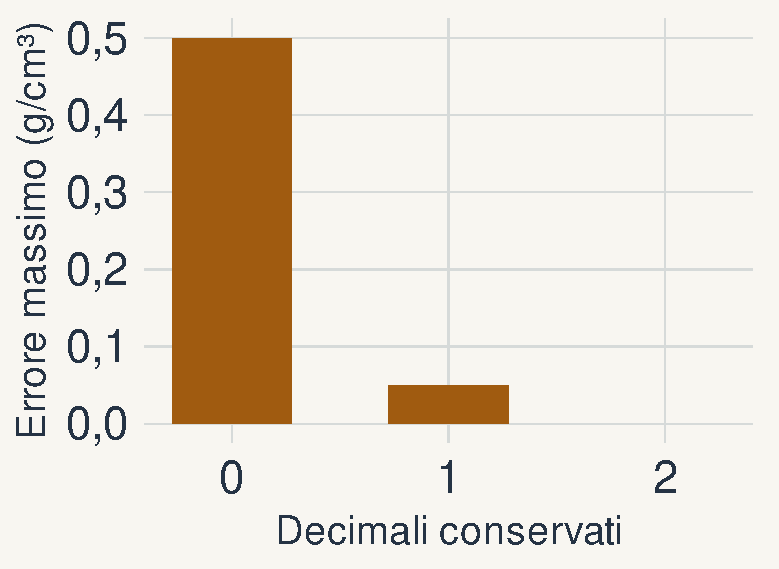
\includegraphics[width=\linewidth,height=6.15cm,keepaspectratio]{Figure/F02.pdf}\par}
\PSmall{Errore massimo introdotto dall’arrotondamento delle densità.}
}};
\node[anchor=north west,inner sep=0] at([xshift=10.85cm,yshift=-2.12cm]current page.north west){\Colonna{8.16cm}{\PBody{Arrotondando le densità a zero, una e due cifre decimali, lo scarto massimo dai valori calcolati è rispettivamente circa 0,5, 0,05 e un residuo dell’ordine della precisione numerica. Il risultato dipende dalla particolare tabella dell’esercizio, nella quale le densità sono costruite con due decimali. La rappresentazione destinata alla lettura può adottare una precisione limitata, mentre gli oggetti utilizzati nei calcoli successivi devono conservare quella necessaria. Una nuova scrittura dei dati arrotondati modificherebbe anche l’impronta del file.}
}};
\end{tikzpicture}\end{frame}

\begin{frame}[plain]\hypertarget{slide14}{}
\bookmark[level=0,page=14]{Piani casuali, versioni e consegna}
\bookmark[level=1,page=14]{Gli indici condivisi definiscono la stessa replica}
\begin{tikzpicture}[remember picture,overlay]
\PilotChrome{Gli indici condivisi definiscono la stessa replica}{PIANI CASUALI, VERSIONI E CONSEGNA}{14}{Per un confronto fra linguaggi, l’identità degli indici è un vincolo più preciso dell’uguaglianza del seme.}
\node[anchor=north west,inner sep=0] at([xshift=.96cm,yshift=-2.12cm]current page.north west){\Colonna{9.40cm}{{\centering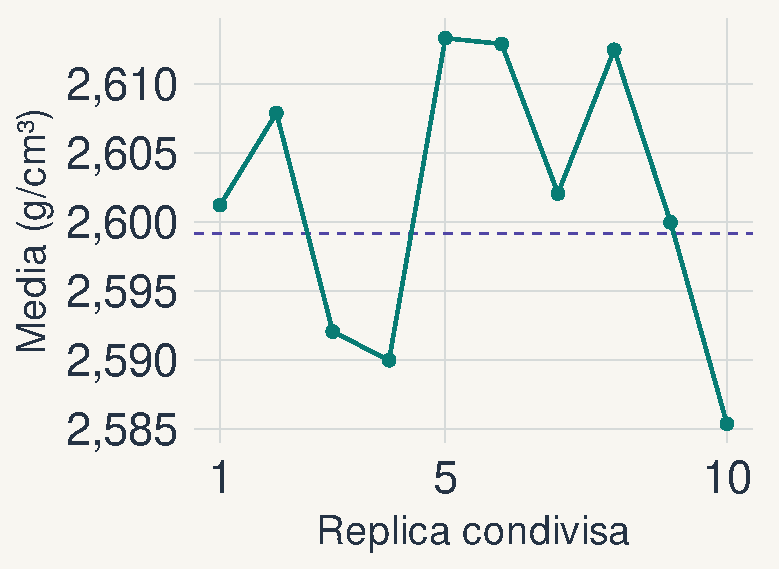
\includegraphics[width=\linewidth,height=6.15cm,keepaspectratio]{Figure/F03.pdf}\par}
\PSmall{Dieci medie su indici condivisi; riferimento: media dei provini.}
}};
\node[anchor=north west,inner sep=0] at([xshift=10.85cm,yshift=-2.12cm]current page.north west){\Colonna{8.16cm}{\PBody{Il progetto conserva dieci piani di ricampionamento, ciascuno composto da ventiquattro indici, e calcola la media delle densità selezionate. L’esempio serve a confrontare implementazioni in R e Python sulle stesse estrazioni, senza assegnare a dieci repliche un ruolo inferenziale. Uno stesso seme numerico non garantirebbe identiche sequenze fra linguaggi o generatori differenti. Il piano esplicito permette di separare l’identità del campione ricostruito dalle differenze di implementazione e di confrontare le medie entro una tolleranza dichiarata.}
}};
\end{tikzpicture}\end{frame}

\begin{frame}[plain]\hypertarget{slide15}{}
\bookmark[level=1,page=15]{La storia Git conserva modifiche ricostruibili}
\begin{tikzpicture}[remember picture,overlay]
\PilotChrome{La storia Git conserva modifiche ricostruibili}{PIANI CASUALI, VERSIONI E CONSEGNA}{15}{Versionare il codice richiede anche riferimenti verificabili alle versioni dei dati e dell’ambiente utilizzati.}
\node[anchor=north west,inner sep=0] at([xshift=.96cm,yshift=-2.12cm]current page.north west){\Colonna{9.40cm}{{\centering\resizebox{0.90\linewidth}{!}{\begin{tikzpicture}[x=1cm,y=-.87cm,every node/.style={font=\fontsize{12.2}{15}\selectfont,text=Ink},arr/.style={-{Stealth[length=2mm]},line width=.8pt,draw=Classical}]\path[use as bounding box] (0,0) rectangle (7.45,6.2);
\draw[draw=Classical,fill=Classical!8,rounded corners=2pt,line width=.7pt] (0.6,1) rectangle (3.2,3);
\node[anchor=center,text=Ink,font=\fontsize{13}{15}\selectfont,text width=2.3cm,align=center] at (1.9,2) {Commit 1: dati};
\draw[arr,draw=Classical] (3.4,2)--(3.9,2);
\draw[draw=Quantum,fill=Quantum!8,rounded corners=2pt,line width=.7pt] (4.1,1) rectangle (6.8,3);
\node[anchor=center,text=Ink,font=\fontsize{12}{15}\selectfont,text width=2.3cm,align=center] at (5.45,2) {Commit 2: dati e analisi};
\node[anchor=center,text=Ink,font=\fontsize{11.5}{15}\selectfont,text width=6.8cm,align=center] at (3.7,4.4) {Ogni stato conserva il proprio antecedente.};
\node[anchor=center,text=Ink,font=\fontsize{11}{15}\selectfont,text width=6.8cm,align=center] at (3.7,5.8) {La storia non incorpora automaticamente i dati esterni.};

\end{tikzpicture}}\par}
}};
\node[anchor=north west,inner sep=0] at([xshift=10.85cm,yshift=-2.12cm]current page.north west){\Colonna{8.16cm}{\PBody{L’esperimento crea un repository temporaneo isolato, registra un primo commit con i dati del provino e un secondo con il calcolo della densità. La storia conserva quindi due stati e il collegamento della modifica al proprio antecedente. La verifica accerta che gli identificativi dei commit siano differenti e che l’albero di lavoro finale sia pulito. La configurazione dell’autore resta locale al repository didattico, mentre nel progetto consegnato vengono conservati lo script riproducibile e il resoconto della storia.}
}};
\end{tikzpicture}\end{frame}

\begin{frame}[plain]\hypertarget{slide16}{}
\bookmark[level=1,page=16]{La consegna rende ricostruibili le dipendenze}
\begin{tikzpicture}[remember picture,overlay]
\PilotChrome{La consegna rende ricostruibili le dipendenze}{PIANI CASUALI, VERSIONI E CONSEGNA}{16}{Una consegna riproducibile esplicita il punto d’ingresso, le dipendenze e i risultati attesi.}
\node[anchor=north west,inner sep=0] at([xshift=.96cm,yshift=-2.12cm]current page.north west){\Colonna{9.40cm}{\PBody{Il pacchetto riunisce dati, funzioni, script principale, estratti delle slide, risultati, informazioni della sessione e resoconto dei controlli. La riesecuzione parte dalla radice del progetto e utilizza percorsi relativi, evitando dipendenze dalla cartella personale dell’autore. Le librerie necessarie vengono dichiarate e controllate prima dell’analisi, senza installazioni implicite durante il calcolo. L’ambiente registrato consente di interpretare differenze dovute alle versioni, mentre le verifiche numeriche aiutano a distinguere una variazione di formattazione da un cambiamento sostanziale del risultato.}
}};
\node[anchor=north west,inner sep=0] at([xshift=10.85cm,yshift=-2.12cm]current page.north west){\Colonna{8.16cm}{\PInfo{R/P10\_funzioni.R definisce il contratto e le trasformazioni. R/P10\_figure.R esegue le prove e produce le figure. La cartella risultati/P10 conserva sintesi, piani, impronte dimostrative e sessione; gli strumenti di verifica ricostruiscono anche il confronto con Python.}
}};
\end{tikzpicture}\end{frame}

\begin{frame}[plain]\hypertarget{slide17}{}
\bookmark[level=1,page=17]{Consegna: dimostrare il procedimento completo}
\begin{tikzpicture}[remember picture,overlay]
\PilotChrome{Consegna: dimostrare il procedimento completo}{PIANI CASUALI, VERSIONI E CONSEGNA}{17}{L’analisi è ricostruibile quando il lettore può eseguire il procedimento e riconoscere le condizioni dei suoi risultati.}
\node[anchor=north west,inner sep=0] at([xshift=.96cm,yshift=-2.12cm]current page.north west){\Colonna{9.40cm}{\PBody{La relazione ricostruisce la densità del primo provino, le medie per stazione e le prove sui dati inammissibili. L’esercizio richiede di spiegare perché file numericamente equivalenti possano avere impronte differenti e perché lo stesso seme non garantisca le medesime estrazioni fra linguaggi. Una modifica controllata introduce un volume nullo e verifica che la procedura si arresti prima della sintesi. La discussione finale collega stabilità del calcolo, integrità dei materiali e condizioni scientifiche dell’analisi, indicando per ciascuna le evidenze disponibili.}
}};
\node[anchor=north west,inner sep=0] at([xshift=10.85cm,yshift=-2.12cm]current page.north west){\Colonna{8.16cm}{\PInfo{La densità del primo provino è 2,68 g/cm³. Il volume nullo deve provocare un errore. Il confronto fra R e Python deve utilizzare gli stessi indici e una tolleranza esplicita: questi tre esiti costituiscono riscontri distinti della consegna.}
}};
\end{tikzpicture}\end{frame}

\begin{frame}[plain]\hypertarget{slide18}{}
\bookmark[level=0,page=18]{Laboratori della spedizione}
\bookmark[level=1,page=18]{Tre fasi della spedizione nel laboratorio}
\begin{tikzpicture}[remember picture,overlay]
\PilotChrome{Tre fasi della spedizione nel laboratorio}{LABORATORI DELLA SPEDIZIONE}{18}{Gli esperimenti usano dati sintetici; la conclusione sul caso resta quella ottenuta dai ventiquattro provini.}
\node[anchor=north west,inner sep=0] at([xshift=.96cm,yshift=-2.12cm]current page.north west){\Colonna{9.40cm}{{\centering\resizebox{0.97\linewidth}{!}{\begin{tikzpicture}[x=1cm,y=1cm,every node/.style={font=\sffamily\fontsize{9.2}{11}\selectfont,text=Ink}]
\node[draw=Classical,fill=Classical,rounded corners=2mm,text=white,text width=2.45cm,align=flush center,minimum height=1.55cm,anchor=west,font=\sffamily\bfseries\fontsize{9.2}{11}\selectfont] (f0) at (0,0.00) {1. Controllare i dati};
\node[draw=Classical!60,fill=Classical!6,rounded corners=1.5mm,line width=.6pt,text width=2.8cm,align=flush center,minimum height=1.55cm,anchor=west] (e00) at (2.95,0.00) {Collegare tabelle senza moltiplicare le misure\\[1pt]{\fontsize{7.6}{9}\selectfont\color{Muted}m02-join}};
\node[draw=Rule,fill=white,rounded corners=1.5mm,line width=.6pt,text width=2.8cm,align=flush center,minimum height=1.55cm,anchor=west] (e01) at (6.10,0.00) {Verificare una tabella analitica\\[1pt]{\fontsize{7.6}{9}\selectfont\color{Muted}m02-tabella}};
\draw[pEdge] (f0.east)--(e00.west);
\node[draw=Classical,fill=Classical,rounded corners=2mm,text=white,text width=2.45cm,align=flush center,minimum height=1.55cm,anchor=west,font=\sffamily\bfseries\fontsize{9.2}{11}\selectfont] (f1) at (0,-1.95) {2. Verificare le funzioni};
\draw[pEdge] (f0.south)--(f1.north);
\node[draw=Classical!60,fill=Classical!6,rounded corners=1.5mm,line width=.6pt,text width=2.8cm,align=flush center,minimum height=1.55cm,anchor=west] (e10) at (2.95,-1.95) {Verificare una funzione prima dell’uso\\[1pt]{\fontsize{7.6}{9}\selectfont\color{Muted}m15-contratti}};
\node[draw=Rule,fill=white,rounded corners=1.5mm,line width=.6pt,text width=2.8cm,align=flush center,minimum height=1.55cm,anchor=west] (e11) at (6.10,-1.95) {Identità e confronto numerico\\[1pt]{\fontsize{7.6}{9}\selectfont\color{Muted}m15-tolleranze}};
\draw[pEdge] (f1.east)--(e10.west);
\node[draw=Classical,fill=Classical,rounded corners=2mm,text=white,text width=2.45cm,align=flush center,minimum height=1.55cm,anchor=west,font=\sffamily\bfseries\fontsize{9.2}{11}\selectfont] (f2) at (0,-3.90) {3. Conservare la provenienza};
\draw[pEdge] (f1.south)--(f2.north);
\node[draw=Classical!60,fill=Classical!6,rounded corners=1.5mm,line width=.6pt,text width=2.8cm,align=flush center,minimum height=1.55cm,anchor=west] (e20) at (2.95,-3.90) {Integrità dei file e identità dei dati\\[1pt]{\fontsize{7.6}{9}\selectfont\color{Muted}m15-integrita}};
\node[draw=Rule,fill=white,rounded corners=1.5mm,line width=.6pt,text width=2.8cm,align=flush center,minimum height=1.55cm,anchor=west] (e21) at (6.10,-3.90) {Parametri, versioni e sensibilità\\[1pt]{\fontsize{7.6}{9}\selectfont\color{Muted}m15-provenienza}};
\draw[pEdge] (f2.east)--(e20.west);
\end{tikzpicture}
}\par}
\PSmall{Fasi della spedizione. Il primo esperimento di ogni fase ha le pagine Scenario A e Confronto.}
}};
\node[anchor=north west,inner sep=0] at([xshift=10.85cm,yshift=-2.12cm]current page.north west){\Colonna{8.16cm}{\PBody{Gli esperimenti ripetono su tabelle sintetiche tre passaggi della spedizione: collegare tabelle senza moltiplicare le misure, verificare il contratto di una funzione, controllare l’integrità di un file. Ogni fase ha uno scenario di partenza e un confronto con un solo parametro modificato.}
\vspace{.2cm}\PLabel{Altri esperimenti delle fasi}
\PLab{https://marzione00.github.io/Lab_Geo/\#laboratorio/m02-tabella}{Verificare una tabella analitica · m02-tabella}
\PLab{https://marzione00.github.io/Lab_Geo/\#laboratorio/m15-tolleranze}{Identità e confronto numerico · m15-tolleranze}
\PLab{https://marzione00.github.io/Lab_Geo/\#laboratorio/m15-provenienza}{Parametri, versioni e sensibilità · m15-provenienza}
}};
\end{tikzpicture}\end{frame}

\begin{frame}[plain]\hypertarget{slide19}{}
\bookmark[level=1,page=19]{Collegare tabelle senza moltiplicare le misure}
\begin{tikzpicture}[remember picture,overlay]
\PilotChrome{Collegare tabelle senza moltiplicare le misure}{LABORATORI DELLA SPEDIZIONE}{19}{Verificare la cardinalità di un collegamento mediante una chiave.}
\node[anchor=north west,inner sep=0] at([xshift=.96cm,yshift=-2.12cm]current page.north west){\Colonna{9.40cm}{{\centering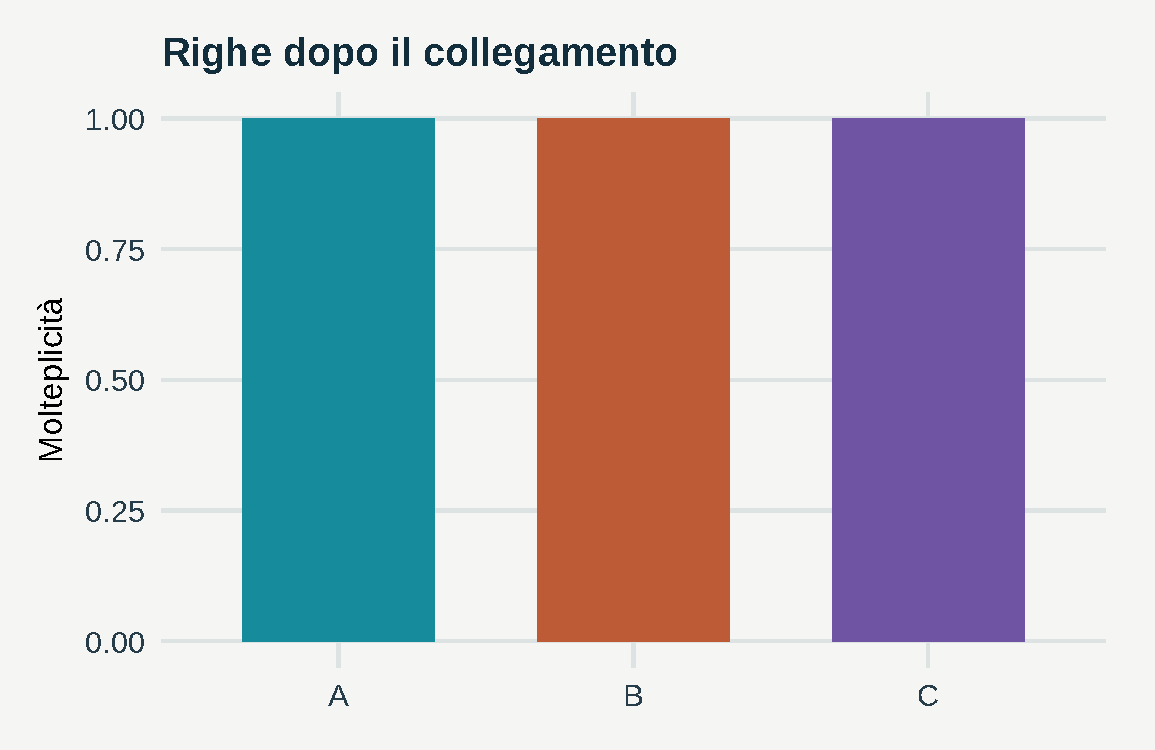
\includegraphics[width=\linewidth,height=6.0cm,keepaspectratio]{Esperimenti/m02-join-A.pdf}\par}
\PSmall{Chiave B nei metadati: Univoca. Seme: 17.}
}};
\node[anchor=north west,inner sep=0] at([xshift=10.85cm,yshift=-2.12cm]current page.north west){\Colonna{8.16cm}{\PLabel{Scenario A · simulazione}
\PBody{Il collegamento associa alle misure una tabella di metadati attraverso l’identificativo della stazione. Quando ciascun identificativo compare una sola volta nei metadati, ogni misura riceve una corrispondenza; introducendo una chiave duplicata, la stessa misura viene ripetuta per ciascuna riga compatibile.}
\par\smallskip{\centering\adjustbox{max width=.98\linewidth}{$\displaystyle n_{\rm join}(k)=n_A(k)n_B(k)$}\par\smallskip}
\PSmall{k è una chiave condivisa; $n_{A}$(k) e $n_{B}$(k) sono le sue occorrenze nelle due tabelle; $n_{join}$(k) conta le combinazioni prodotte dal collegamento.}
}};
\node[anchor=north east,inner sep=0] at([xshift=17.1cm,yshift=-12.04cm]current page.north west){\fontsize{7.7}{9}\selectfont \href{https://marzione00.github.io/Lab_Geo/\#laboratorio/m02-join}{\color{Classical}\bfseries Apri il laboratorio · m02-join}};
\end{tikzpicture}\end{frame}

\begin{frame}[plain]\hypertarget{slide20}{}
\bookmark[level=1,page=20]{Confronto | Collegare tabelle senza moltiplicare le misure}
\begin{tikzpicture}[remember picture,overlay]
\PilotChrome{{\fontsize{15.3}{19}\selectfont Confronto | Collegare tabelle senza moltiplicare le misure}}{LABORATORI DELLA SPEDIZIONE}{20}{Una chiave duplicata può replicare le osservazioni e modificarne il peso.}
\node[anchor=north west,inner sep=0] at([xshift=.96cm,yshift=-2.12cm]current page.north west){\Colonna{9.40cm}{{\centering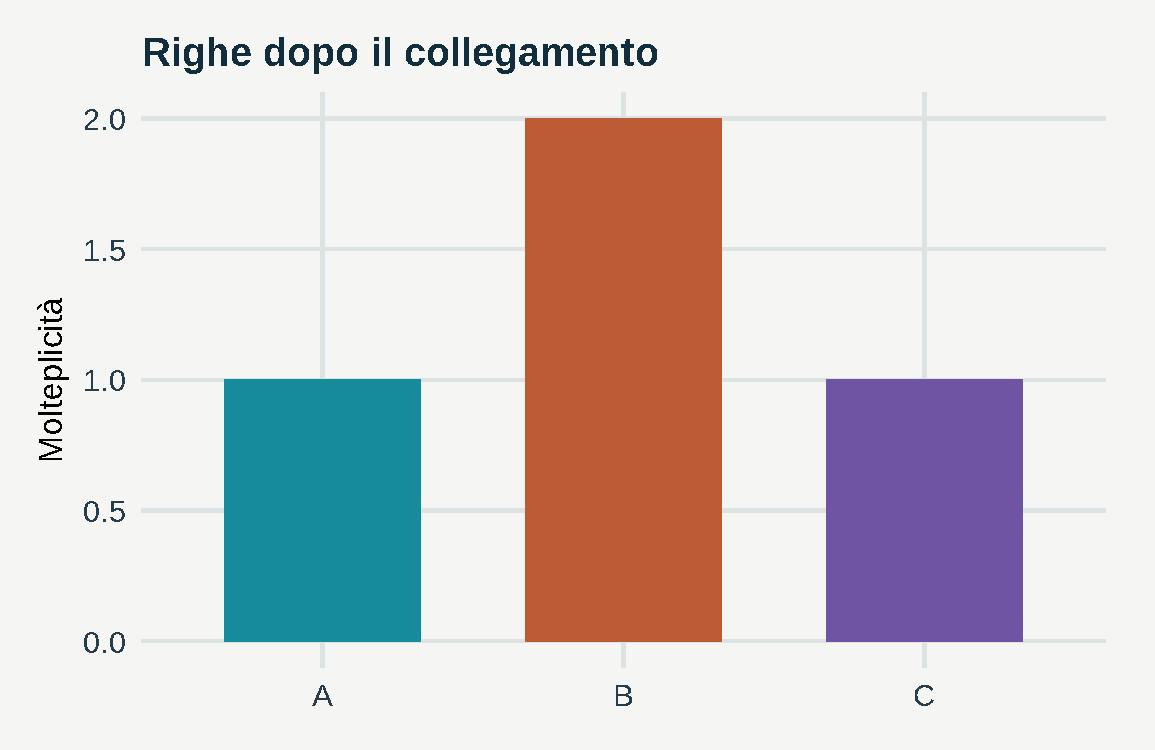
\includegraphics[width=\linewidth,height=5.6cm,keepaspectratio]{Esperimenti/m02-join-B.pdf}\par}
\PSmall{Chiave B nei metadati: Univoca $\to$ Duplicata. Tutti gli altri parametri e il seme sono fissi.}
}};
\node[anchor=north west,inner sep=0] at([xshift=10.85cm,yshift=-2.12cm]current page.north west){\Colonna{8.16cm}{\PLabel{Confronto fra gli scenari}
{\fontsize{10.2}{12.8}\selectfont\begin{tabular}{@{}>{\raggedright\arraybackslash}p{0.48\linewidth}@{\hspace{.13cm}}>{\raggedright\arraybackslash}p{0.224\linewidth}@{\hspace{.13cm}}>{\raggedright\arraybackslash}p{0.224\linewidth}@{}}\toprule Grandezza & A & B\\[2.3pt]
\midrule 
Righe iniziali & 3 & 3\\[2.3pt]
Righe finali & 3 & 4\\[2.3pt]
Media iniziale & 5,33 & 5,33\\[2.3pt]
Media dopo join & 5,33 & 5,25\\[2.3pt]
\bottomrule\end{tabular}\par}
\vspace{.25cm}\PBody{Con una chiave duplicata nei metadati le righe passano da 3 a 4 e la media dopo il collegamento scende da 5,33 a 5,25, perché una misura entra due volte. Il conteggio delle righe prima e dopo il collegamento rivela l’errore.}
}};
\node[anchor=north east,inner sep=0] at([xshift=17.1cm,yshift=-12.04cm]current page.north west){\fontsize{7.7}{9}\selectfont \href{https://marzione00.github.io/Lab_Geo/\#laboratorio/m02-join}{\color{Classical}\bfseries Apri il laboratorio · m02-join}};
\end{tikzpicture}\end{frame}

\begin{frame}[plain]\hypertarget{slide21}{}
\bookmark[level=1,page=21]{Verificare una funzione prima dell’uso}
\begin{tikzpicture}[remember picture,overlay]
\PilotChrome{Verificare una funzione prima dell’uso}{LABORATORI DELLA SPEDIZIONE}{21}{Sottoporre una funzione a casi validi e invalidi.}
\node[anchor=north west,inner sep=0] at([xshift=.96cm,yshift=-2.12cm]current page.north west){\Colonna{9.40cm}{{\centering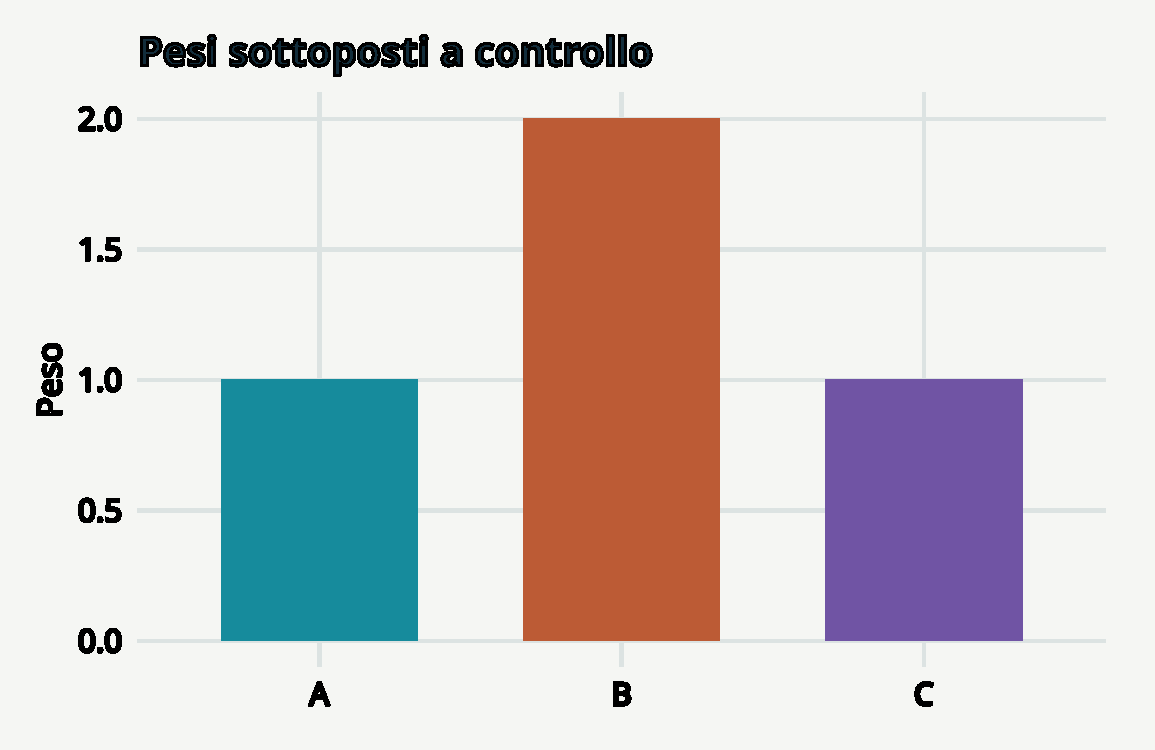
\includegraphics[width=\linewidth,height=6.0cm,keepaspectratio]{Esperimenti/m15-contratti-A.pdf}\par}
\PSmall{Caso di controllo: Pesi validi. Seme: 17.}
}};
\node[anchor=north west,inner sep=0] at([xshift=10.85cm,yshift=-2.12cm]current page.north west){\Colonna{8.16cm}{\PLabel{Scenario A · simulazione}
\PBody{Il contratto di una funzione specifica le condizioni nelle quali il risultato possiede il significato previsto. L’esperimento considera una media pesata con pesi finiti, non negativi e somma positiva. Le configurazioni disponibili permettono di confrontare un ingresso valido con pesi che violano una o più condizioni, mentre la carta rende visibile il vettore sottoposto a verifica.}
\par\smallskip{\centering\adjustbox{max width=.98\linewidth}{$\displaystyle \bar x_w=\frac{\sum_iw_ix_i}{\sum_iw_i},\quad w_i\ge0,\quad\sum_iw_i>0$}\par\smallskip}
\PSmall{$x_i$ è il valore dell’osservazione i e $w_i$ il peso assegnato. La media pesata divide la somma dei prodotti $w_i x_i$ per la somma dei pesi; il dominio qui dichiarato richiede $w_i$$\geq$0 e somma strettamente positiva.}
}};
\node[anchor=north east,inner sep=0] at([xshift=17.1cm,yshift=-12.04cm]current page.north west){\fontsize{7.7}{9}\selectfont \href{https://marzione00.github.io/Lab_Geo/\#laboratorio/m15-contratti}{\color{Classical}\bfseries Apri il laboratorio · m15-contratti}};
\end{tikzpicture}\end{frame}

\begin{frame}[plain]\hypertarget{slide22}{}
\bookmark[level=1,page=22]{Confronto | Verificare una funzione prima dell’uso}
\begin{tikzpicture}[remember picture,overlay]
\PilotChrome{Confronto | Verificare una funzione prima dell’uso}{LABORATORI DELLA SPEDIZIONE}{22}{I controlli esplicitano il dominio della funzione e distinguono errori d’ingresso da risultati ammessi.}
\node[anchor=north west,inner sep=0] at([xshift=.96cm,yshift=-2.12cm]current page.north west){\Colonna{9.40cm}{{\centering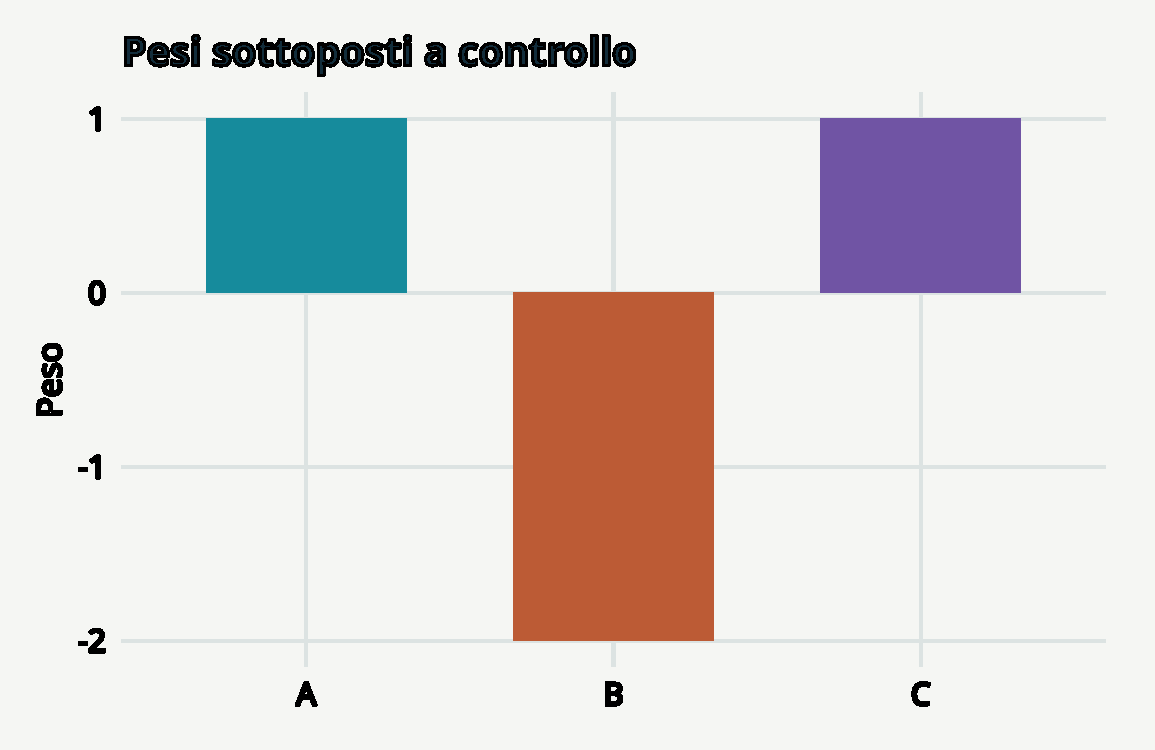
\includegraphics[width=\linewidth,height=5.6cm,keepaspectratio]{Esperimenti/m15-contratti-B.pdf}\par}
\PSmall{Caso di controllo: Pesi validi $\to$ Un peso negativo. Tutti gli altri parametri e il seme sono fissi.}
}};
\node[anchor=north west,inner sep=0] at([xshift=10.85cm,yshift=-2.12cm]current page.north west){\Colonna{8.16cm}{\PLabel{Confronto fra gli scenari}
{\fontsize{10.2}{12.8}\selectfont\begin{tabular}{@{}>{\raggedright\arraybackslash}p{0.48\linewidth}@{\hspace{.13cm}}>{\raggedright\arraybackslash}p{0.224\linewidth}@{\hspace{.13cm}}>{\raggedright\arraybackslash}p{0.224\linewidth}@{}}\toprule Grandezza & A & B\\[2.3pt]
\midrule 
Pesi non negativi & sì & no\\[2.3pt]
Somma positiva & sì & no\\[2.3pt]
Risultato & 5,25 & Input respinto dal contratto\\[2.3pt]
\bottomrule\end{tabular}\par}
\vspace{.25cm}\PBody{Un peso negativo fa fallire il controllo del dominio. Il rifiuto è l’esito previsto per un ingresso incompatibile con la media pesata definita.}
}};
\node[anchor=north east,inner sep=0] at([xshift=17.1cm,yshift=-12.04cm]current page.north west){\fontsize{7.7}{9}\selectfont \href{https://marzione00.github.io/Lab_Geo/\#laboratorio/m15-contratti}{\color{Classical}\bfseries Apri il laboratorio · m15-contratti}};
\end{tikzpicture}\end{frame}

\begin{frame}[plain]\hypertarget{slide23}{}
\bookmark[level=1,page=23]{Integrità dei file e identità dei dati}
\begin{tikzpicture}[remember picture,overlay]
\PilotChrome{Integrità dei file e identità dei dati}{LABORATORI DELLA SPEDIZIONE}{23}{Confrontare contenuto numerico, rappresentazione testuale e impronta di un file.}
\node[anchor=north west,inner sep=0] at([xshift=.96cm,yshift=-2.12cm]current page.north west){\Colonna{9.40cm}{{\centering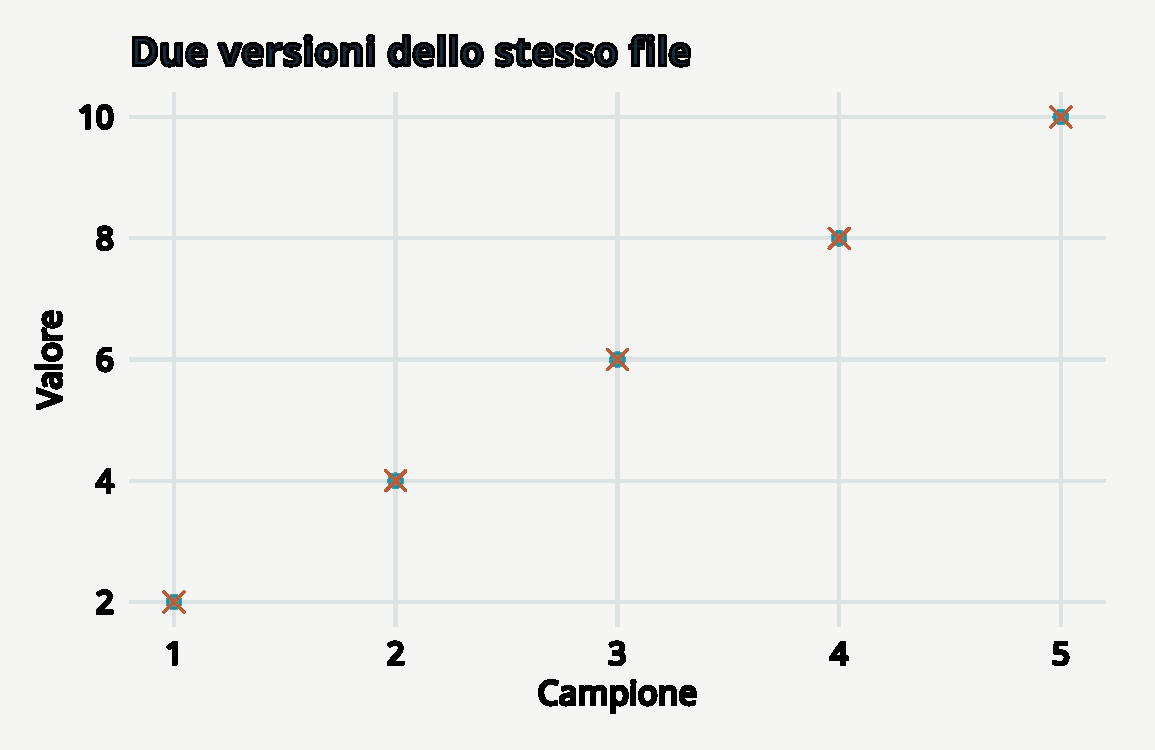
\includegraphics[width=\linewidth,height=6.0cm,keepaspectratio]{Esperimenti/m15-integrita-A.pdf}\par}
\PSmall{Variazione dell’ultima misura: 0. Seme: 17.}
}};
\node[anchor=north west,inner sep=0] at([xshift=10.85cm,yshift=-2.12cm]current page.north west){\Colonna{8.16cm}{\PLabel{Scenario A · simulazione}
\PBody{L’attività scrive due tabelle in file CSV temporanei, dopo avere applicato alla seconda una variazione controllata dell’ultima misura. Vengono quindi confrontati valori numerici, sequenze di byte e impronte MD5, rendendo esplicito il passaggio dalla tabella in memoria al contenuto persistente.}
\par\smallskip{\centering\adjustbox{max width=.98\linewidth}{$\displaystyle D_A=D_B\Longrightarrow h(D_A)=h(D_B)$}\par\smallskip}
\PSmall{$D_A$ e $D_B$ sono le sequenze di byte dei due file; $h$ è la funzione di impronta. L’implicazione scritta procede dall’identità dei file all’uguaglianza delle impronte.}
}};
\node[anchor=north east,inner sep=0] at([xshift=17.1cm,yshift=-12.04cm]current page.north west){\fontsize{7.7}{9}\selectfont \href{https://marzione00.github.io/Lab_Geo/\#laboratorio/m15-integrita}{\color{Classical}\bfseries Apri il laboratorio · m15-integrita}};
\end{tikzpicture}\end{frame}

\begin{frame}[plain]\hypertarget{slide24}{}
\bookmark[level=1,page=24]{Confronto | Integrità dei file e identità dei dati}
\begin{tikzpicture}[remember picture,overlay]
\PilotChrome{Confronto | Integrità dei file e identità dei dati}{LABORATORI DELLA SPEDIZIONE}{24}{La ricostruzione conserva il file effettivamente analizzato e documenta quando il suo contenuto cambia.}
\node[anchor=north west,inner sep=0] at([xshift=.96cm,yshift=-2.12cm]current page.north west){\Colonna{9.40cm}{{\centering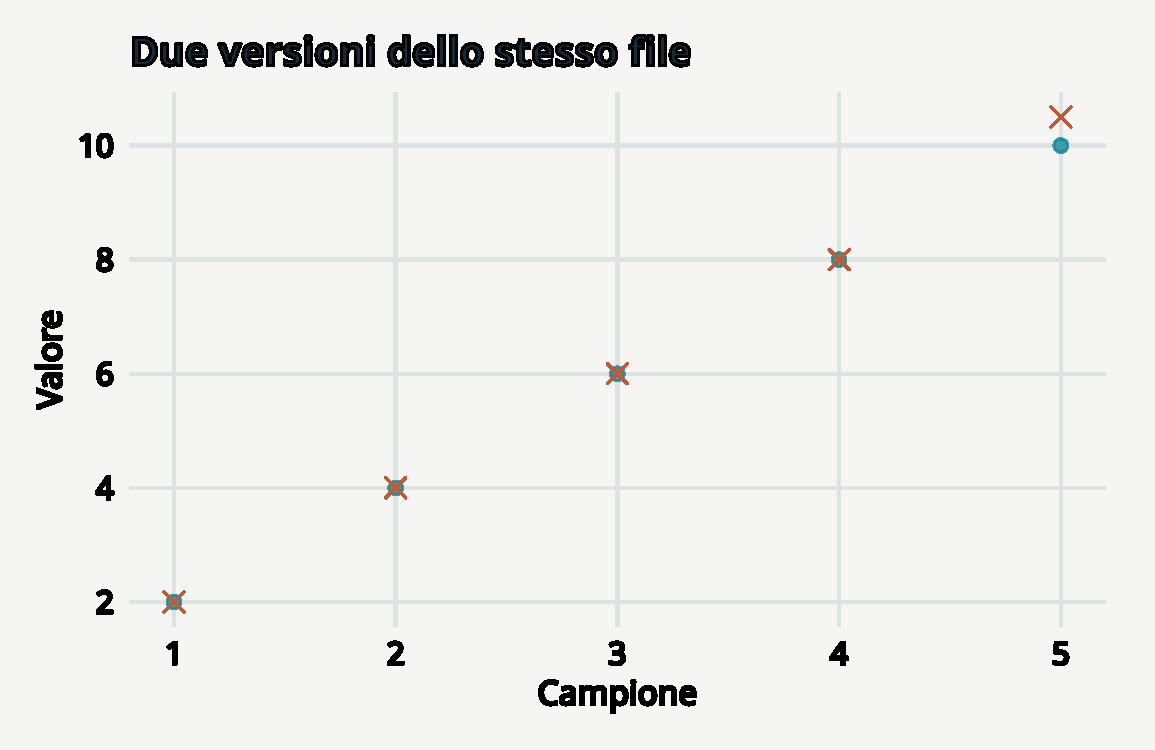
\includegraphics[width=\linewidth,height=5.6cm,keepaspectratio]{Esperimenti/m15-integrita-B.pdf}\par}
\PSmall{Variazione dell’ultima misura: 0 $\to$ 0,5. Tutti gli altri parametri e il seme sono fissi.}
}};
\node[anchor=north west,inner sep=0] at([xshift=10.85cm,yshift=-2.12cm]current page.north west){\Colonna{8.16cm}{\PLabel{Confronto fra gli scenari}
{\fontsize{10.2}{12.8}\selectfont\begin{tabular}{@{}>{\raggedright\arraybackslash}p{0.48\linewidth}@{\hspace{.13cm}}>{\raggedright\arraybackslash}p{0.224\linewidth}@{\hspace{.13cm}}>{\raggedright\arraybackslash}p{0.224\linewidth}@{}}\toprule Grandezza & A & B\\[2.3pt]
\midrule 
Byte identici & sì & no\\[2.3pt]
Impronta A & eb826a… & eb826a…\\[2.3pt]
Impronta B & eb826a… & 406e5e…\\[2.3pt]
Scarto numerico massimo & 0 & 0,5\\[2.3pt]
\bottomrule\end{tabular}\par}
\vspace{.25cm}\PBody{Con una variazione di 0,5, la seconda impronta cambia e lo scarto numerico diventa osservabile. Le impronte sono usate qui per confrontare copie didattiche.}
}};
\node[anchor=north east,inner sep=0] at([xshift=17.1cm,yshift=-12.04cm]current page.north west){\fontsize{7.7}{9}\selectfont \href{https://marzione00.github.io/Lab_Geo/\#laboratorio/m15-integrita}{\color{Classical}\bfseries Apri il laboratorio · m15-integrita}};
\end{tikzpicture}\end{frame}

\begin{frame}[plain]\hypertarget{slide25}{}
\bookmark[level=1,page=25]{Dal risultato alla relazione}
\begin{tikzpicture}[remember picture,overlay]
\PilotChrome{Dal risultato alla relazione}{SINTESI}{25}{Consegna dati, codice, controlli, sessione e storia insieme al risultato, con percorsi relativi.}
\node[anchor=north west,inner sep=0] at([xshift=.96cm,yshift=-2.12cm]current page.north west){\Colonna{9.40cm}{\PLabel{Domanda di partenza}
\PBody{Che cosa serve perché un’analisi semplice possa essere rieseguita e verificata da altri?}
\PLabel{Risultato da discutere}
\PBody{La densità media dei ventiquattro provini è circa 2,599 g/cm³, con medie di stazione da 2,513 a 2,685. I controlli interrompono l’elaborazione per ciascuno dei cinque input inammissibili, e due file che contengono lo stesso valore scritto in due modi producono impronte diverse.}
}};
\node[anchor=north west,inner sep=0] at([xshift=10.85cm,yshift=-2.12cm]current page.north west){\Colonna{8.16cm}{\PLabel{Limiti della conclusione}
\PBody{Ottenere di nuovo lo stesso numero dimostra la stabilità del procedimento dichiarato. La validità della misura di densità e della conclusione geologica dipende dalla definizione del problema e dal protocollo di raccolta.}
\vspace{.4cm}\href{https://marzione00.github.io/Lab_Geo/\#modulo-P11}{\color{Classical}\bfseries Prosegui · P11 · Classificare nuove stazioni sintetiche}
}};
\end{tikzpicture}\end{frame}

\begin{frame}[plain]\hypertarget{slide26}{}
\bookmark[level=1,page=26]{Fonti, dati e codice per riprodurre le figure}
\begin{tikzpicture}[remember picture,overlay]
\PilotChrome{Fonti, dati e codice per riprodurre le figure}{RIFERIMENTI}{26}{I risultati numerici si riferiscono ai dati e alle ipotesi dichiarate nel caso.}
\node[anchor=north west,inner sep=0] at([xshift=.96cm,yshift=-2.12cm]current page.north west){\Colonna{9.40cm}{\PLabel{Dati e attribuzioni}
\PBody{Dati del corso (campioni\_modulo1.csv e numeri casuali comuni): massa e volume di ventiquattro provini di sei stazioni. Funzioni, controlli, impronte e storia Git sono costruiti nella spedizione.}
}};
\node[anchor=north west,inner sep=0] at([xshift=10.85cm,yshift=-2.12cm]current page.north west){\Colonna{8.16cm}{\PLabel{Nell’archivio dei sorgenti}
\PBody{Codice contiene i frammenti delle pagine; R contiene lo script P10\_figure.R, che ricostruisce figure e valori dai dati. Esperimenti comprende i programmi dei due scenari, Diagrammi i disegni TikZ modificabili, Scena il modello Blender della copertina.}
\vspace{.4cm}\href{https://marzione00.github.io/Lab_Geo/\#modulo-P10}{\color{Classical}\bfseries Apri la spedizione P10 su GeoStat Lab}
}};
\end{tikzpicture}\end{frame}
\end{document}
